\section{Libreria JaCaMo}

In questa sezione viene descritta la liberia realizzata per JaCaMo mostrando la struttura e le componenti.

\subsection{Struttura}

\begin{figure}[H]
\centering
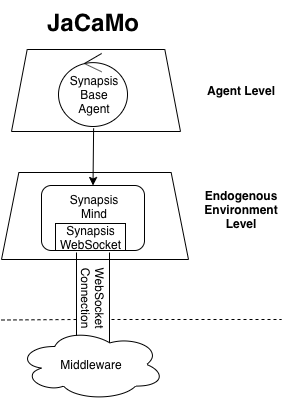
\includegraphics[width=0.5\linewidth]{figures/struttura_libreria_JaCaMo.png}
\caption{Struttura libreria per JaCaMo}
\label{JaCamo_synapsis}
\end{figure}

L'immagine \ref{JaCamo_synapsis}, simile alla figura \ref{livelli_jacamo} che illustrava i livelli del framework JaCaMo, mostra la composizione della libreria realizzata per mettere in comunicazione il Sistema Multi-Agente con Synapsis.

\subsection{Artefatto Synapsis} \label{artefatto_synapsis}

L'artefatto è risultato il componente più adatto (sezione \ref{struttura_nuova_entita}), lato MAS, per realizzare l'effettivo collegamento, tramite WebSocket, al middleware. All'interno dell'artefatto \textit{Synapsis Mind} sono presenti le funzionalità per gestire la WebSocket, per inviare azioni (in forma di messaggi strutturati) e ricevere le percezioni inviate da Synapsis.

\begin{figure}[H]
\centering
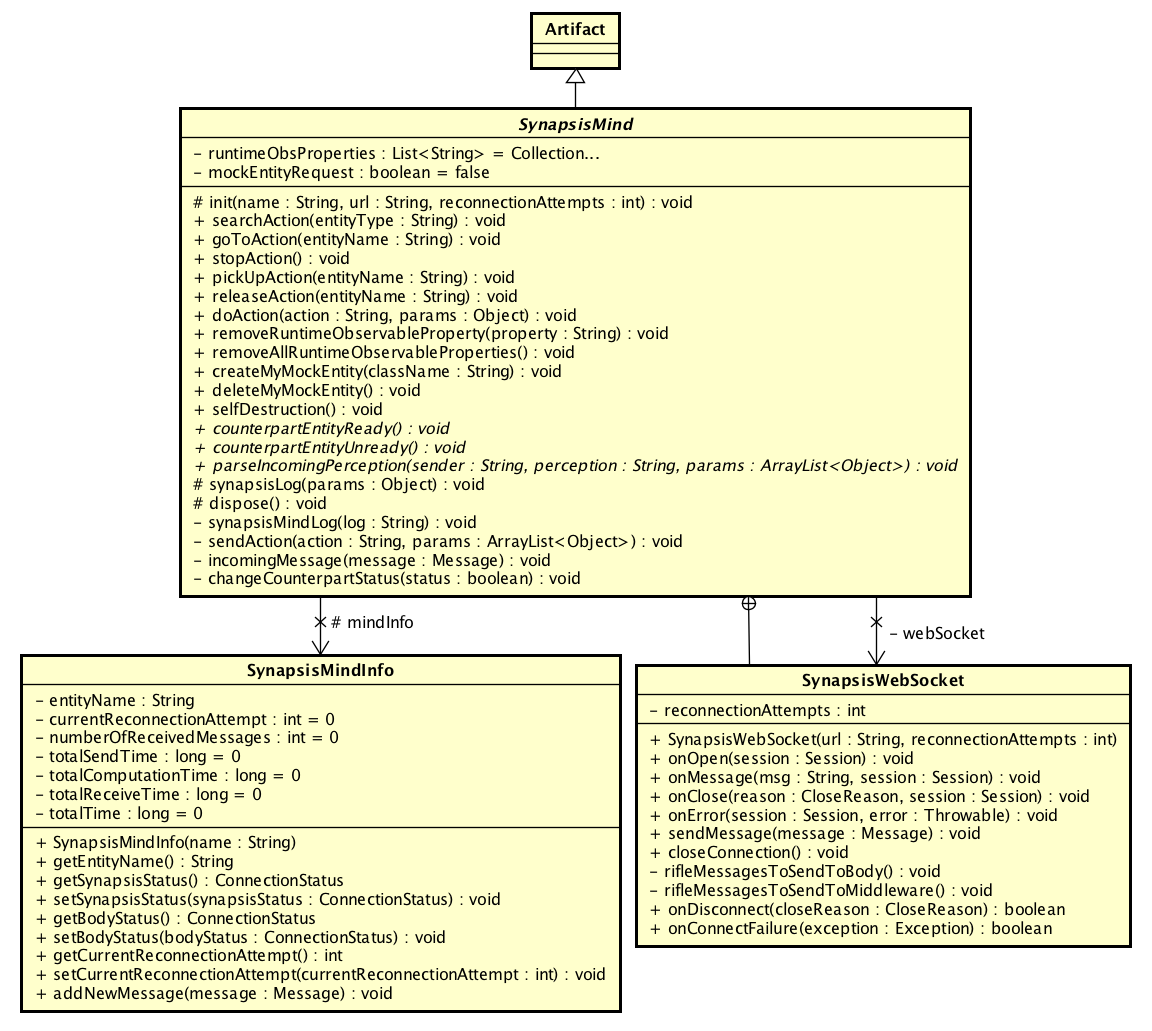
\includegraphics[width=\linewidth]{figures/diagramma_classi_artefatto.png}
\caption{Diagramma delle classi per l'artefatto synapsis}
\label{classi_artefatto}
\end{figure}

Nella figura \ref{classi_artefatto} è presente la struttura della classe \textit{SynapsisMind} che estende \textit{Artifact}, rendendola a tutti gli effetti un artefatto per il MAS. Il metodo \textit{incomingMessage(message)} viene invocato ad ogni messaggio ricevuto dal middleware e si occupa di aggiungere il contenuto del messaggio alle proprietà osservabili dell'artefatto, notificando l'agente collegato dell'arrivo di una nuova percezione. 

\medskip

Sono stati realizzati diversi metodi, che abilitano la mente a comunicare con il corpo attraverso l'utilizzo della notazione \textit{@OPERATION}, ad esempio \textit{doAction(action,params)} che permette l'invio di una generica azione. La notazione \textit{@OPERATION} è la modalità definita su CArtAgO per definire le operazioni (metodi) utilizzabili dall'agente. I restanti metodi, presenti nel listato \ref{synapsisMindActions}, sono stati realizzati perché presentano azioni comuni a molti scenari, oltre a quello scelto come esempio (sezione \ref{caso_studio}) e delineano azioni predefinite già collegate ad effettive attività che il corpo è stato reso in grado di svolgere (vedere la sezione \ref{libreria_unity}).

\lstinputlisting[label={synapsisMindActions},caption={Operazioni (azioni) disponibili all'agente},language=Java]{code/SynapsisMind_Actions.java}

\medskip

All'interno di \textit{SynapsisMind} è presente la classe \textit{SynapsisWebSocket} con l'obiettivo di gestire tutte le funzionalità associate al protocollo WebSocket, messe a disposizione dalla liberia Tyrus \cite{tyrus}. Computazionalmente l'utilizzo di una WebSocket genera un processo separato rispetto al flusso computazionale di CArtAgO, per questo motivo è stato fatto uso delle API, \textit{beginExternalSession} e \textit{endExternalSession}, presenti nell'artefatto che permettono di realizzare metodi utilizzabili da processi esterni.

\medskip

Per collegarsi al middleware è necessario definire a quale indirizzo è attivo Synapsis. \'E l'agente che riceve questa informazione durante il processo di inizializzazione dell'artefatto. Per approfondimenti consultare l'appendice. 

\medskip

La classe \textit{SynapsisMindInfo} contiene le informazioni necessarie ad identificare l'entità rappresentata, lo stato del collegamento al middleware e lo stato di collegamento con l'entità "corpo" sulla Game Engine.

\subsection{Agente Synapsis}

L'agente \textit{Synapsis Base Agent} contiene le funzionalità (beliefs e plans) basilari per la realizzazione di un agente predisposto a Synapsis.

\lstinputlisting[label={synapsisBaseAgent},caption={Agente Base Synapsis},language=asl]{code/synapsis_base_agent.asl}

Il listato \ref{synapsisBaseAgent} mostra beliefs e plans necessari all'agente per istanziare il proprio artefatto SynapsisMind. Il belief \textit{synapsis\_base\_name("synapsis\_"} è utilizzato per identificare, all'interno del MAS, gli artefatti istanziati utilizzando questa libreria. La parte restante del nome dell'artefatto è direttamente collegato al nome dell'agente, quindi, nel caso l'agente si chiami \textit{robot}, il proprio artefatto sarà nominato \textit{synapsis\_robot}.

\medskip

Il plan \textit{+synapsis\_counterpart\_status(Name,C)} ha lo scopo di "notificare" l'agente dello stato di collegamento alla controparte "corpo", sia in caso di connessione che di disconnessione. Attraverso \textit{+!createSynapsisMind(Params)} e \textit{+!createSynapsisMind} è possibile istanziare il proprio artefatto. Il primo plan permette la realizzazione di un artefatto con parametri aggiuntivi rispetto a quelli predefiniti.

\medskip

Per realizzare agenti specifici è quindi necessario utilizzare \textit{Synapsis Base Agent} come agente base dal quale prendere beliefs e plans. Nell'appendice \ref{appendice_JaCamo} è presente una spiegazione più dettagliata del procedimento da seguire.


